\chapter{Background}
\label{ch2}
In this chapter an overview of power systems is presented followed by a description of supervised and reinforcement learning concepts. Finally, the literature review is proposed.

\section{Power system}
\label{sec:2ps}
Nowadays, electricity is given for granted and that flipping the switch will turn the light on instantly and effortless. But electricity performs a long journey before arriving to houses or where it is consumed. To reach its destination, electricity circulates in power networks or power systems.\\
\subsection{Description of a power system}
%https://www.generatorsource.com/Articles/Generator-Info/High-Medium-and-Low-Voltage-Differences.aspx
%Power systems are facilities that produce and transport electricity to consumers. \\

A power system is a complex infrastructure that produces and distributes electricity to different consumers. A power network consists of generation, transmission and distribution system and each of them has a different function. \\

%Power transmission systems consist of an interconnected set of overhead lines, cables and related equipment that are used for the transfer of electricity at high voltage levels between supply points and load points, such as customers and other electric systems. \\

In the traditional power system, electricity is generated in large, centralised power plants. The electricity is then transferred to the loads using the transmission and distribution networks. Transmission substations are located near the power plants. Their main function is to increase the voltage level to high and extra-high voltages levels. The reason for power transmission at high and extra-high voltage levels is to increase efficiency. The lower current that accompanies high-voltage transmission allows thinner and lighter cables to be used. This reduces the construction costs of towers and power lines. In Belgium, high and extra-high voltages refer to voltage magnitudes $36 kV \leq |V| < 380 kV$ for the high voltage and $|V| \geq 380 kV$ for the extra high voltage \cite{elia}. \\
Large industrial complexes and factories that require a substantial amount of power often utilise medium supply voltages. The high voltage coming from the transmission lines is sent to the primary substation, this can supply step-down power to secondary substations or to single buildings. Secondary substations can have transformers to further step-down the power, and they are generally located in areas that can serve one or more buildings. Medium voltages refer to voltage magnitude $6 kV \leq |V| < 36 kV$. \\
Then the medium supply power is step down again to a low voltage and sent to the domestic household or home appliances power supply. Low voltages refer to voltage magnitude $|V| < 6 kV$. \\
\begin{figure}[H]
\centering
    % 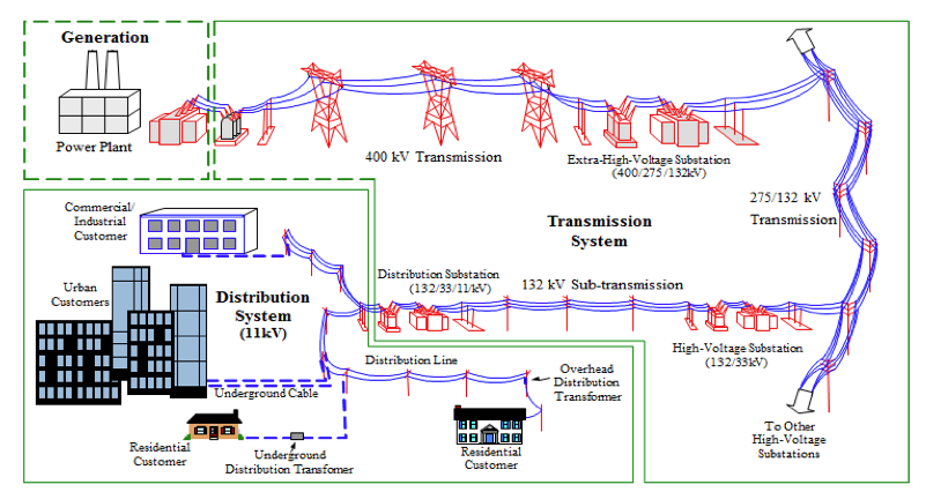
\includegraphics[width=.9\linewidth]{images/DN/HighMediumLowV.png}
    % 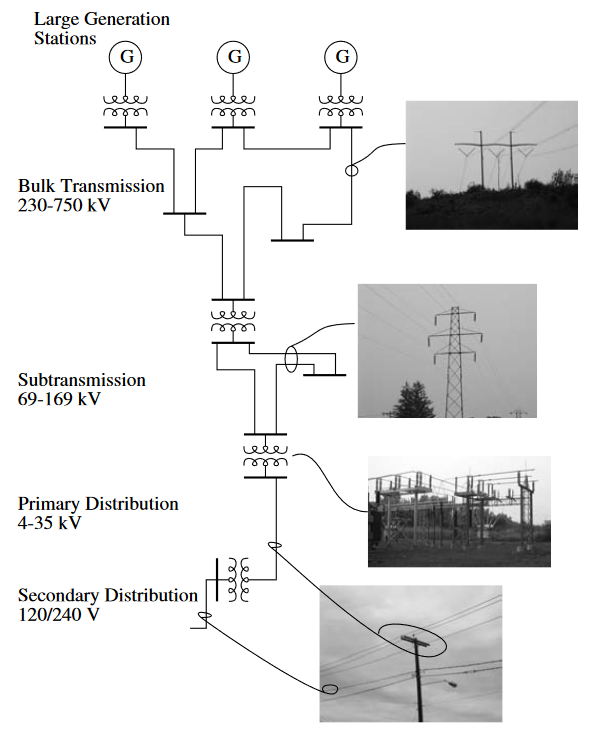
\includegraphics[width=.25\linewidth]{images/Background/DN/DN.PNG}
    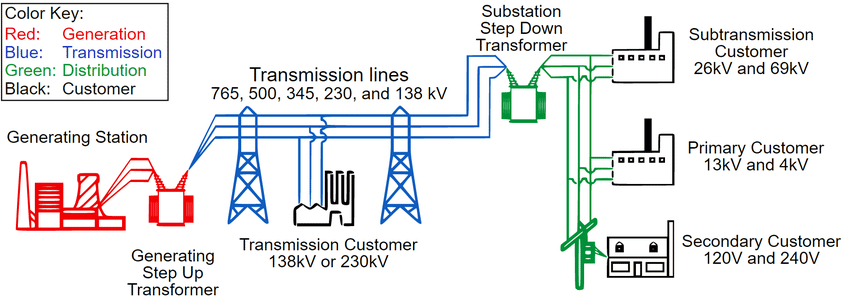
\includegraphics[width=.9\linewidth]{images/Background/DN/Basic-Structure-of-the-Electric-Power-System-5.png }
\caption[Power network distribution]{Typical Power network distribution \cite{USblackout}.}
% \label{fig:}
\end{figure}


\noindent These power networks include many elements and devices that are needed to generate, transport and assure that there are no problems in a network.\\
These elements are: \label{networkeledesc}
\begin{itemize}
    \item \textbf{Generator}. These generate electricity starting from a different form of energy. In general, electricity is produced when a magnet rotates within closed loops of wire to create a steady flow of electrons.\\
    For this reason, many generators produce energy using turbines: a fluid spins the generator's blades, producing electricity. This fluid, either water or air, can derive from natural sources: hydroelectric, wind or geothermal turbines, or generated by combustion of some fuel, for example coal, natural gas, oil or nuclear source. \\
    There are other generators that do not need a turbine to generate electricity, for example solar panels.
    
    \item \textbf{Lines}. These transport the power from where energy is generated to where it is consumed. These lines have to be long enough to reach any destination. One of the main issues about transportation lines is insulation. \\
    There are different types of lines: overhead cables, they use air to insulate the bare conductors, or underground cables. For latter cables, particular attention must be taken to insulate them from other conductors and from the earth (ground). Also, the material used must be resistant to damages, corrosion, and it must avoid that the water is being absorbed.
    
    \item \textbf{Transformers}. Transformers are used to interlink systems operating at different voltages. These can increase  the voltage magnitude near a generator power plant or decrease it near the consumptions facilities. \\
    Changing the voltage magnitude allows reducing the power loss due to transportation. One of the main causes of power loss is the Joule effect: some part of the energy transmitted is converted in heat generated by the current flowing through a conductor. This power lost is given by the equation $P=RI^2$, where \gls{R} is the resistance and \gls{I} is the current through a line, so decreasing the current reduces the energy loss.
    
    % \item \textbf{Switchgear}. In an electricity supply, it is necessary to disconnect equipment from the network quickly if a fault occurs to avoid damage on the elements of the network, or to disconnect some points of the network to avoid excessive losses or too high or low voltages. \\
    % Switchgear is a broad term that describes a wide variety of switching devices that fulfil the need of controlling, protecting, and isolating power systems. Among these switching devices the most common are: \emph{circuit breaker}, during an electrical fault, a circuit breaker will detect the anomaly and interrupt the power flow, effectively limiting damage to the system; \emph{switch} is an electrical component that can disconnect or connect the conducting path in an electrical circuit, interrupting the electric current or diverting it from one conductor to another; \emph{recloser} similar to the circuit breaker but used in high voltage networks, these devices handle trouble temporary occurrences such as lightning, windblown tree branches or wires,
    % birds, or rodents damaging the wires.
    
    \item \textbf{Loads}. These are electric components that consume the electric power generated by power plants. The types of loads can be divided base on the consumption in:
    \begin{itemize}
        \item[] \emph{Domestic loads}, the domestic loads mainly consist of lights, fan, refrigerator, air conditioners, mixer, grinder, heater, ovens, small pumping, motor, etc. The domestic loads consume very little power.
        \item[] \emph{Commercial loads}, the commercial loads mainly consist of lightning, fans, heating, air conditioning and many other electrical appliances used in establishments such as markets, restaurants, shops. This type of load consumes energy for more hours during the day as compared to the domestic load.
        \item[] \emph{Industrial loads}, the industrial loads refer from a small-scale industry, to a heavy industry. Industrial loads may be connected during the whole day \cite{EDNdesign}.
    \end{itemize}
    
    % \item Load buses where \gls{P} and \gls{Q} are specified.
    % \item Generator buses where the voltage magnitude \gls{V} and the power \gls{P} are specified.
    % \item A primary bus, an "infinite" bus, where the magnitude voltage \gls{V} is specified (normally 1 \gls{pu}) and its phase angle \gls{Vangle} is assumed to be zero as a reference angle. At this bus, both \gls{P} and \gls{Q} can be what is needed to keep the network stable. \cite{eps}
\end{itemize}

\subsection{Power flow}
\label{ssec:powerflow}
%Mathmatical formulation: https://www.engineering.iastate.edu/~jdm/ee458_2011/PowerFlowEquations.pdf
%Simple discussion: https://www.pterra.com/power-flow-analysis/power-flow-solution-techniques/
An important procedure in power systems is to perform a numerical analysis to determine the electrical state of the network, starting from some parameters that are known. This analysis is called power flow (\gls{PF}).\\
The objective of a \gls{PF} study is to calculate the voltages, magnitude and angle, for a given bus, load, generation device. After this information is known for all elements, line flows and losses can be calculated.\\

A bus is a node of the network where a line or several lines are connected to. Loads and generators can be connected to it as well. There are different types of bus:
\begin{itemize}
    \item \emph{Slack bus}. It is taken as a bus reference, where the magnitude and phase angle of the voltage are specified. Slack bus magnitude considers 1 \gls{pu} and the phase angle 0 of degrees. This bus provides the additional real and reactive energy to cover the demand.

    \item \emph{Load bus or PQ bus}. At these buses, the real and reactive powers are specified. The buses' magnitude and phase angles are unknown until the final solution is obtained.

    \item \emph{Voltage controlled bus or PV bus}. Instead, at these buses, the real power and voltage magnitude are specified, and the phase angles of the voltages and the reactive power are known only after the final solution is obtained. The limits on the value of reactive power are also specified. 
\end{itemize}
%The \gls{PF} is an optimization problem essential for planning purposes: besides the calculation of electrical characteristics of the power system, power flow analysis can also help to optimize the system operating conditions, minimize the power losses and determine control actions to satisfy the demand while meeting operational constraints.

% \subsubsection{Buses}
% The power flow gives information about the steady state of the entire system such as voltage, active, reactive power and lines' loading.\\
% Each bus is associated with four quantities: voltage magnitude \gls{V}, phase angle \gls{angleV}, real power \gls{AP} and reactive power \gls{Q}.
% Depending on the quantity that has been specified, buses in the power system are classified into the following three different types:
% \begin{itemize}
%     \item \textbf{Slack bus}. It is taken as reference where the magnitude and phase angle of the voltage are specified. Slack bus magnitude considers 1 \gls{pu} and phase angle 0 degrees. This bus provides the additional real and reactive power to supply the transmission losses, since there are unknown until the final solution is obtained.

%     \item \textbf{Load buses or PQ bus}. At these buses, the real and reactive powers are specified. The magnitude and phase angle of the bus voltage are unknown until the final solution is obtained.

%     \item \textbf{Voltage controlled buses or PV bus}. At these buses, the real power and voltage magnitude are specified. The phase angles of the voltages and the reactive power are unknown until the final solution is obtained. The limits on the value of reactive power are also specified. 
% \end{itemize}

\subsubsection{Solution techniques}
Defining and solving the \gls{PF} equations are the main tasks in load flow analysis. \\
The definition of the \gls{PF} equations is based on Ohm’s Law, which is the relationship between voltages and currents. For a network, it can be expressed in matrix notation as follows:
\[
    \mathbf{I} = \mathbf{Y} \times \mathbf{V}
\]
% \[
%  \begin{bmatrix}
%  Y_{1,1} & Y_{1,2} & \quad & \cdots & \quad & Y_{1,N-1} & Y_{1,N} \\
%  & & & & & & \\
%  Y_{2,1} & Y_{2,2} & \quad & \cdots & \quad & Y_{2,N-1} & Y_{2,N} \\
%  & & & & & & \\
 
%  \vdots & \vdots & \quad & \ddots & \quad & \vdots & \vdots \\
%  & & & & & & \\
 
%  Y_{N-1,1} & Y_{N-1,2} & \quad & \cdots & \quad & Y_{N-1,N-1} & Y_{N-1,N} \\
%  & & & & & & \\
%  Y_{N,1} & Y_{N,2} & \quad & \cdots & \quad & Y_{N,N-1} & Y_{N,N} \\
%  \end{bmatrix}
%  \times
%  \begin{bmatrix}
%  V_1 \\ \\ V_2 \\ \\ \vdots \\ \\ V_{N-1} \\ \\ V_N
%  \end{bmatrix}
%  =
%  \begin{bmatrix}
%  I_1 \\  \\ I_2 \\ \\ \vdots \\ \\ I_{N-1} \\ \\ I_N
%  \end{bmatrix}
% \]

\noindent Where:
\begin{itemize}
    \item \textbf{Y} is the bus admittance matrix
    \item \textbf{V} is an array of bus voltages
    \item \textbf{I} is an array of bus current injections %(positive value when generation, and negative value when load)
\end{itemize}

The \gls{PF} formulation is based on the application of Kirchhoff’s laws to meshed electric networks. The concept of the \glf{PF} calculation is that the sum of all flows into each node is equal to the sum of flows flowing out.\\
The flows equations are in complex form, they consist of real and reactive components. That means that if there are n nodes, then there are n complex equations. 
%The resulting system of equations involves non-linear relationships, making the calculations not easy.
Solution methods for this system of equations are primarily iterative with the objective of reducing the sum of flows in all nodes to some acceptably small value known as the mismatch tolerance. \\

All these iterative methods follow the same basic concept: they assume starting values for the dependent variables, primarily voltage at nominal voltage magnitude (i.e. 1 \gls{pu}) and zero phase angle; compute new values for those voltages using the nodal network equation or a numerical approximation and repeat until the convergence criteria are met.

% The solution has to satisfy some network constrains, in particular:
% \begin{itemize}
%     \item Active and reactive power balance: the sum of the power injections (that can be positive or negative) at each bus must be equal to 0. This, as said, results from the Kirchhoff’s laws.
    
%     \item Voltage limits: the voltage magnitude at each bus and the voltage phase difference between two directly connected buses are bounded by some specific values to maintain the system safe.
    
%     \item Thermal limits on transmission lines: the flow in each transmission line is limited due to the thermal limit of the conductors.
    
%     \item Generators' active and reactive power limits: the generating units have generally a minimum and maximum level of output power.
    
%     \item Generator ramping limits: the output power of a generating unit can not be instantaneously increased or decreased. The operator must take into account the ramping limits of the generators.
% \end{itemize}

\subsubsection{Convergence}
The \gls{PF} is a non-linear and non-convex numerical analysis, with a large number of constraints and variables. It is, therefore, a hard problem, whose cost of finding a solution can increase exponentially, particularly with the increasing size of the network. Moreover, there is no guarantee to find the global optimum. \\
When a solution exists, and it is reached, it is said that the network has converged. The calculation has converged when all nodes have met the mismatch tolerance. \\
The main \gls{PF} solution methods are:
\begin{itemize}
    \item Gauss-Seidel method updates the voltage one node at a time until all nodes are within the mismatch tolerance.
    
    \item Newton-Raphson method uses a first order expansion of the \gls{PF} equations to approach convergence. It is generally faster than the Gauss-Seidel method and able to converge to small tolerances. This method is prone to \textbf{divergence}, when mismatches increase instead of decrease from iteration to iteration. This occurs when the solution vector exits outside the feasible solution space at any point during the algorithm. As soon as the solutions are outside the feasible space, the gradient tends to further increase mismatches, leading to solutions that “blow-up” in the numerical sense.\\
    This method requires calculating the first order approximation matrix, known as the Jacobian.
    % Several variations on the Newton-Raphson are in use, including:
        % \begin{itemize}
        %     \item[] Fast Decoupled: separates the loosely linked real and reactive components of the power flow equations in order to speed up solution.
        %     \item[] Fixed Newton: does not update the first order approximation matrix every iteration to reduce computational burden.
        %     \item[] Non-divergent power flow: applies a reduction to the Jacobian multiplier whenever the solution appears to exit feasible space. In certain situations, this may prevent divergence, or at least stop it before blow-up.
        % \end{itemize}
    \item Interior-Point Newton method forces the solution inside feasible space to avoid divergence. The interior point method uses a second order expansion of the \gls{PF} equations to find a solution. The method is more computationally intensive than either the Gauss-Seidel or Newton-Raphson, but is less susceptible to numerical divergence \cite{pfmethods}.
\end{itemize}

\subsubsection{Divergence}
Divergence is the condition of the power network when the numerical solution can not be found any more due to some possible issues:

\begin{itemize}
    \item the power system is going to “blow-up.”
    \item the power system is in voltage collapse.
    \item the power system is unstable.
    \item the initial conditions defined were bad or poor.
    \item some issues related to software or input data.
\end{itemize}

Divergence of the \gls{PF} solution is usually associated with the singularity of the Jacobian matrix. Since some methods require an inverse of the Jacobian as part of its solution algorithm, singularity of the Jacobian means division by zero \cite{eps}.

\subsection{Voltage problems in power systems}
The power systems are highly secure, but they are far from perfect, and some issues may arise at any moment, for example voltage problems. Voltage problems arise when the voltage through a line or a device is more or less than what it is expected. These cases should be handled correctly. There are two voltage problems that can raise on a network: under and over voltage problems.\\
Generally, electronic devices have defined voltage limits to work in safety conditions. The voltage magnitude in the different parts of a network is not always constant during time, but it fluctuates. These fluctuations, both positive and negative, can be large: when negative, the voltage can drop below the device's minimum allowed voltage limit, in this case there would be an under voltage problem; or when positive, the voltage can increase above its maximum, in this case there would be an over voltage problem. \\

The voltage control problem has been studied for years, but it only came under the spotlight in the last years for the increasing number of distributed resources introduced in the networks. \\
%https://www.electricalindia.in/overvoltage-mitigation-techniques-for-pv-grid/
The introduction of more and more \gls{DER} devices in the networks increases the number of voltages problems, in particular over voltage problems. These devices generate electric power and when this power is greater than the energy consumed, the extra energy is emitted back in the network.\\

For this reason, it is important to control the voltage in an electrical power system for a regular operation of the electrical equipments. It can prevent damages such as overheating of devices and lines, reduce transmission losses and maintain the ability of the system to last and avoid voltage collapses. Over voltages other than shorten the lifetime of equipments have a negative impact on the stable operation of both supply side devices and demand-side appliances. \\

% %phd report
% %https://roadnighttaylor.co.uk/news/what-is-active-network-management/
% %Curtailment + curtailment % + solution/compensations
% %https://windeurope.org/wp-content/uploads/files/policy/position-papers/WindEurope-Priority-Dispatch-and-Curtailment.pdf
A possible way to control and manage the voltage on the network to avoid voltage problems and to ensure its stability is active network management (\gls{ANM}). Indeed, the principle of \gls{ANM} is to address congestion and voltage issues via short-term decision making policies \cite{ANMQuentin}. \\
\gls{ANM} creates a smarter network infrastructure providing automated control of various components in the network and provides the information needed to ensure that every device performs in an optimal manner. This control allows grid companies to avoid the traditional approach of reinforcing the network with expensive upgrades; so reducing the costs.
For example, in case of energy generation, from the renewable devices, higher than what a particular line can handle, a grid company, to avoid congestions and possible overvoltages, has three main options:
\begin{itemize}
    \item Replace the existing line with a line that can handle a higher voltage. This usually means replacing the existing line with a cable with a larger cross-sectional area.
    \item Add another parallel line.
    \item Handle the situation with \gls{ANM}.
\end{itemize}
The first two solutions require some infrastructure investment that can be expensive and troublesome, especially in the case of overhead or underground lines.\\
The solution with \gls{ANM} does not require construction cost for the grid company; to keep the network working, in this case, the output of the renewable devices can be curtailed, or the reactive power modulated to reduce lines' overloading. \\

% In these references, generally, \gls{ANM} maintains the system within operational limits by relying on the curtailment of the generator devices, \glspl{PV}, \glspl{WP} and other \gls{DER} devices. \\
% Curtailment of renewable energy may be seen as counter-intuitive on the environmental point of view, and it may be considered as last option. Indeed, this process can slow down the switch to clean energy, because of the lost of the curtailed energy. \\

% In this mindset, \gls{ANM} could also be used to control different elements in the grid to reduce the curtailment power waste: 
% \begin{itemize}
%     \item Flexible loads, also known as virtual batteries, such as water heaters, air conditioning systems, electric vehicles, can be controlled to be turned on if the energy production is higher than the energy consumption so to avoid curtailment on the generators \cite{flexibleloads}.
%     \item use Flexible Alternating Current Transmission System (\gls{FACTS}) devices. They offer some level of power flow control and enhance the transfer capability over the existing network. This flexibility can be utilized for congestion mitigation and renewable energy integration. Particularly, \gls{FACTS} devices allow controlling all parameters that determine active and reactive power transmission: nodal voltages magnitudes and angles and line reactance. These devices replace the mechanical switches with semiconductor switches allowed much faster response times. One problem with these devices is the cost a system operator should sustain to implement them in the network \cite{facts}.
%     % \item Controlling generators' active and reactive power using smart inverters.
% \end{itemize}

%https://electrical-engineering-portal.com/how-reactive-power-is-helpful-to-maintain-a-system-healthy
% It is therefore required to take some actions to avoid these over voltages situations. In particular, it is useful and sometimes needed to reduce the output of renewable generators to prevent possible voltage problems. This means that the output power of these generators is less from what they could otherwise have produced given the available resources. Such prevention is often referred to as the process of curtailment. Said generation curtailment, along with storage and transmission losses, constitute the principal sources of energy loss that could be minimised with smart control system like active network management \gls{ANM} \cite{gym-anm}. \\

\noindent The control voltage problem has some interesting properties:
\begin{itemize}
    \item It is a combination of local and global problems: the voltage at each node is influenced by the powers of all other nodes, but the impact depends on the distance between them.
    
    \item It is a constrained optimisation problem with many constraints, for example to keep the voltage in a given range, and the objective is to minimise the total power loss.
    
    \item Voltage control has a relatively large tolerance, and there are no severe consequences if the control fails to meet the requirements for short periods of time. \cite{wang2022multiagent}
    
    \item It is a hierarchical problem where the information available can be represented as a pyramid: much information is available at the top of the pyramid (distribution stations and substations) and it decreases at the base of the pyramid (houses, factories) mainly due to the absence of many sensors.
\end{itemize}


% \subsection{Power system reliability}
% \label{sec:psr}
% %https://info.ornl.gov/sites/publications/Files/Pub57467.pdf
% Reliability of a power system is an important factor concerning the quality of energy supply. \\
% Power reliability can be defined as the degree to which the performance of the elements in a system results in electricity being delivered to customers within accepted standards and in the desired amount \cite{MPRPQ}. \\
% Reliability indices typically consider such aspects as:
% \begin{itemize}
%  \item the number of customers;
%  \item the connected loads;
%  \item the duration of the interruption measured in seconds, minutes, hours, or days;
%  \item the amount of power interrupted;  
%  \item and the frequency of interruptions.
% \end{itemize}

% These factors depend on variable such as reliability of individual items of equipment, circuit length and loading, network configuration, distribution automation, and available transfer capacity \cite{EDNdesign}. \\

% For reliability purposes, it is important to know the maximum voltage that can be
% transferred with transmission lines to meet the anticipated load demand. It is also important to know the levels of power through various transmission lines under certain contingency outage conditions to maintain the continuity of service. Knowledge of power flows and voltage levels under normal operating conditions are necessary in order to determine fault currents and the ensuing consequences on the stability of the system \cite{eps}. \\

% \noindent There exists some standards about power system reliability. \\
% The International Electrotechnical Commission (\gls{IEC}), IEC TS 62749 \cite{iec}, that states that the energy suppliers and facility managers need to verify the conformity of the energy supplied to:
% \begin{itemize}
%     \item maximum limits
%     \item statistical limits over a week or a year
% \end{itemize}
% \noindent Under normal operating condition some values must be verified:
% \begin{itemize}
%     \item during each period of one week $95\%$ of the 10 minutes mean \gls{rms} values of the supply power voltage shall be within the range of $\pm10\%$ \gls{pu} and
%     \item all 10 minutes mean \gls{rms} values of the supply voltage shall be within the range $+10\% \/ -15\%$ \gls{pu}
% \end{itemize}

% The American National Standards Institute (\gls{ANSI}), C84.1-2016 \cite{ansic84}, voltage standards for service voltage limits, for example, are classified as Range A and Range B limits. The voltage between $0.950$ \gls{pu} and $1.050$ \gls{pu} of nominal voltage lies under Range A, and the voltage between $0.917$ \gls{pu} and $1.058$ \gls{pu} of nominal voltage for $240$ \gls{V} service voltage lies under Range B. Note that the voltage can be within Range B for only a short duration and frequency, and thus corrective measures are necessary to constrict.

% %Determining power flow requires measurements of some power system conditions; utilities measure a combination of quantities such as voltage magnitude \gls{V}, real power \gls{P} and reactive power \gls{Q} of the elements connected to the network. 

% \subsubsection{Reliability criteria}
% \label{ssec:n1cri}
% The goal of a distribution system operator (\gls{DSO}) is to ensure a reliable system. Unfortunately, a completely reliable electricity supply is not feasible to obtain since it comes at an infinite cost. So, network operators need to determine an acceptable reliability level, by balancing the costs and benefits, where acceptable reliability level means that all the elements in a network have an acceptable voltage range. \\

% The European \gls{GARPUR} project (\textbf{G}enerally \textbf{A}ccepted \textbf{R}eliability \textbf{P}rinciple with \textbf{U}ncertainty modelling and through probabilistic \textbf{R}isk assessment) developed reliability management approaches and criteria. One of these criteria used by system operators is the N-1 criterion. \\

% The basic principle of N-1 security in network planning states that if a component, for example a transformer or circuit, should fail or be shut down in a network operating at the maximum levels of transmission and supply, the network security must still be guaranteed. This means that the safety of the system is guaranteed and the spreading of the failure is avoided. \\
% It is possible that there may be another contingency before restoring the network after the fail of one element, this criterion is known as N-1-1 criterion.  \\

% With the increasing of network complexity more than one element may fault, for this reason there exists other levels of reliability, like the N-2 criteria. In this case, even if in the network two components fail, the network security is guaranteed. \\
% This N-2 criteria requires much more computational power since, the system operator must calculate what happens to the network for any combination of two fault elements. So, the problem becomes a combination problem, where the possible combination are given by: $N \choose 2$, with $N$ the number of elements in the network. \\

% In general, the calculation can be extended to any generic $k$ elements, but the complexity of the problem increases with the value of $k$. Indeed, the possible combination in a N-k contingency are: $N \choose k$, with $2 < k < N$

% \section{Power system voltage managment}

% \section{Pandapower}
% \label{ch:pandapower}
% This thesis project will be developed with the help of Pandapower. \\
% Pandapower is a Python based power system analysis tool aimed at automation of static and quasi-static analysis and optimization of power systems \cite{pandapower}. \\
% Pandapower is a powerful tool that allows to easily create a model for any power network using customizable predefined data structures, it can solve the \gls{PF} problems, perform the state estimates, topological graph searches and diagnose the system for possible errors.

% \subsection{Data structure}
% Pandapower is based on a tabular data structure, where every element is represented by a table that holds all parameters for a specific component. It is possible to add more information at the data structure, indeed, after the calculation of the power flow, a result table, which contains the element specific results of the different analysis methods, is added to the structure. \\
% The tabular data structure is based on the Python library pandas. It allows storing variables of any data type, so that electrical parameters can be stored together with status variables and meta-data, such as names or descriptions. The tables can be easily expanded and customized by adding new columns without influencing the Pandapower functionality. All inherent pandas methods can be used to efficiently read, write and analyse the network and results data. \\

% A Pandapower network is a Python dictionary that holds all information about the network. Most importantly, it includes element and a result tables for each element type, such as line, transformer, switch, loads. The element table holds all input parameters that are specified by the user, while the result table is used to store the results of the power flow calculation. Input and output parameters are identified by the same index in both tables \cite{pandapower}.

% \begin{figure}[H]
% \centering
%     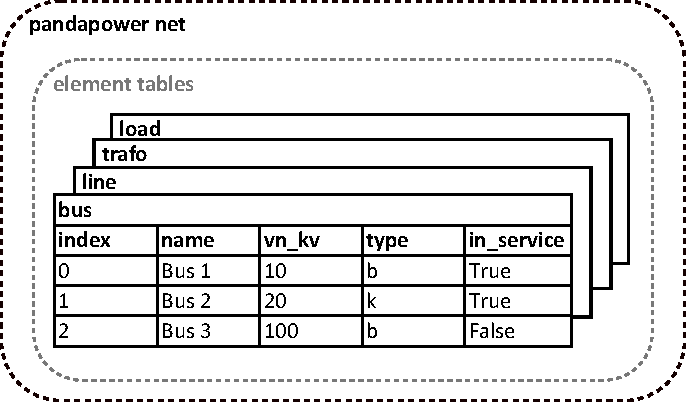
\includegraphics[width=.6\linewidth]{images/Background/Pandapower/Pandapower_net.pdf}
% \caption[Pandapower data frame]{Pandas data frame representation of the Pandapower network}
% % \label{fig:gym_anm_net}
% \end{figure}


% \subsection{Network models}
% Pandapower allows to use different type of elements.

% \subsection{Network models}
% There are two main ways of how a power system can be defined by a user.
% A commonly used approach is the bus-branch model (\gls{BBM}), which defines the network as a collection of buses which are connected by generic branches. Branches are modelled with a predefined equivalent circuit and are used to model multiple elements connected to that branch (multi-pole), like lines or transformers. Buses are attributed with power injections to model single-pole elements like loads, generators or capacitor banks. Since the \gls{BBM} is an accurate mathematical representation of the network, electric equations for power systems analysis can be directly derived from it, but the need to calculate the impedances for each branch and to sum power injections at each bus manually can be cumbersome and error-prone, especially for complex elements. \\
% Instead of a \gls{BBM}, Pandapower uses an element-based model (\gls{EBM}) to model electric grids. An element is either connected to one or multiple buses and is defined with characteristic parameters. This allows defining the network parameters, such as length and relative impedance for lines, or short circuit voltage and rated apparent power for transformers. While \gls{BBM} allows only the definition of a summed power injection at each bus, single-pole elements (such as load or generation elements) can be connected to buses independently. This also allows connecting multiple elements at one bus. The element models are then processed internally with the appropriate equivalent \gls{BBM} circuits to derive a mathematical description of the grid \cite{pandapower}. This decoupling the element model from the electric model allows specifying different equivalent circuits for different analysis functionalities. For example, an external grid element can be modelled as a slack node in the power flow calculation, but as a voltage source with internal impedance in the short circuit calculation.

% \subsection{Power flow solver}
% As said, power flow is one of the most important electric analysis function for power system planning. It allows calculating the current flows and voltages in the network. \\
% The Pandapower power flow solver is based on the Newton-Raphson method. The implementation is based on PYPOWER Python library. To solve the \gls{PF}, the bus constraints include maximum and minimum voltage magnitude, active and reactive power limits can be defined for PV and slack-elements like external grids and generators, but also for PQ-elements, such as loads and static generators. \\
% % After defining all the network elements, to run the power flow solver it is just need to execute the command: 

% % \begin{algorithm}[h]
% % \state pandapower.runpp(net, ...)
% % \end{algorithm}

% After running the power flow calculation, new tables are added to the network data frame.
% \begin{figure}[H]
% \centering
%     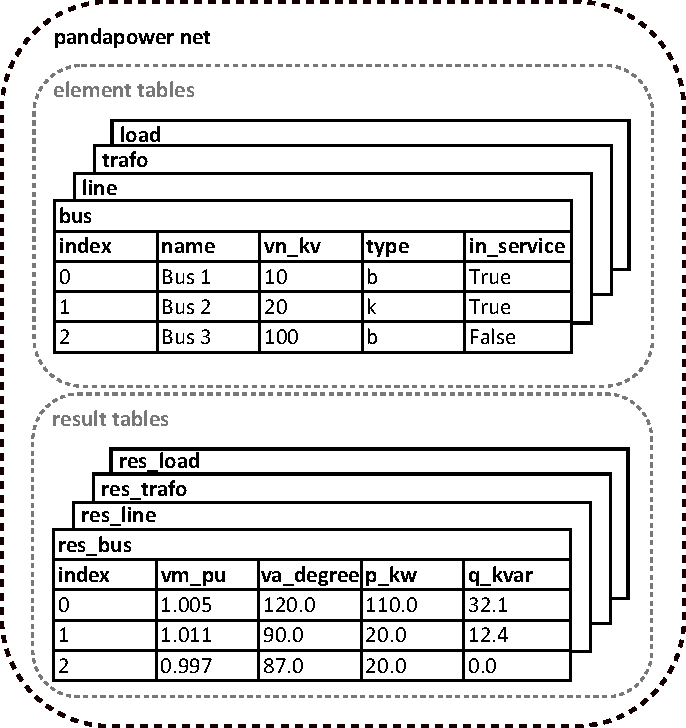
\includegraphics[width=.6\linewidth]{images/Background/Pandapower/Pandapower_resnet_big.pdf}
% \caption[Pandapower data frame (after the power flow calculation)]{Pandas data frame representation of the Pandapower network after the power flow calculation}
% % \label{fig:gym_anm_net}
% \end{figure}

% The power flow calculation on a Pandapower network can fail to converge for a vast variety of reasons, which often makes debugging difficult, annoying and time-consuming. To help with that, the diagnostic function automatically checks Pandapower networks for the most common issues leading to errors. It provides logging output and diagnoses with a controllable level of detail.

%%% SAD :'( %%%
% \noindent this function takes as input the Pandapower network data structure and some other optional values (for example the algorithm solver, max number of iterations, tolerance and so on). \\

% \noindent Internally, Pandapower solves the following optimization problem:

% \begin{align*}
%     \min &\sum_{i \: \in \: gen, sgen, load, external grid} P_i \cdot f(P_i) \\
%         \textrm{s.t.} \\
%         & \text{load flow equations} \\
%         & \text{branch constraints} \\
%         & \text{bus constraints} \\
%         & \text{operation power flow equations}
% \end{align*}

% \noindent where $P_i$ is the active power of any element and $f()$ is the cost function. Few example of the possible constrains are: 
% \begin{align*}
%         & P_{min,i} \leq P_{g} \le P_{max,i}, \; g \in gen \\
%         & Q_{min,i} \leq Q_{g} \le Q_{max,i}, \; g \in gen \\
%         & V_{min,i} \leq V_{g} \le V_{max,i}, \; i \in bus
% \end{align*}

% \noindent It is possible to customize the cost function and choosing between a piece-wise or polynomial cost function. Detailed information about the optimization problem, cost function and network constrains are available in the Pandapower documentation \cite{pandapower2}. \\

% \subsection{Time series}
% Pandapower allow running time series analysis for a given network. There are two main requirements for time series calculations:
% \begin{itemize}
%     \item a Pandapower network
%     \item some time series (in a panda's data frame for example)
% \end{itemize}

% To execute the time series calculation, the loads, generators and other elements' active and reactive power time series have to be passed to a controller that will be in charge to change the elements' values according to the time series. \\

% The time series calculation can be run with the command: 
% \begin{algorithm}[h]
% \state pandapower.timeseries.run\_time\_series.run\_timeseries(net, ...)
% \end{algorithm}

% \noindent this command will start a loop that iterates over every \textbf{time\_step}. For each step, a control loop is started for each controller by \textbf{run\_control}. The controller updates the elements' values at each step with the values given in the time series.

% \begin{figure}[H]
% \centering
%     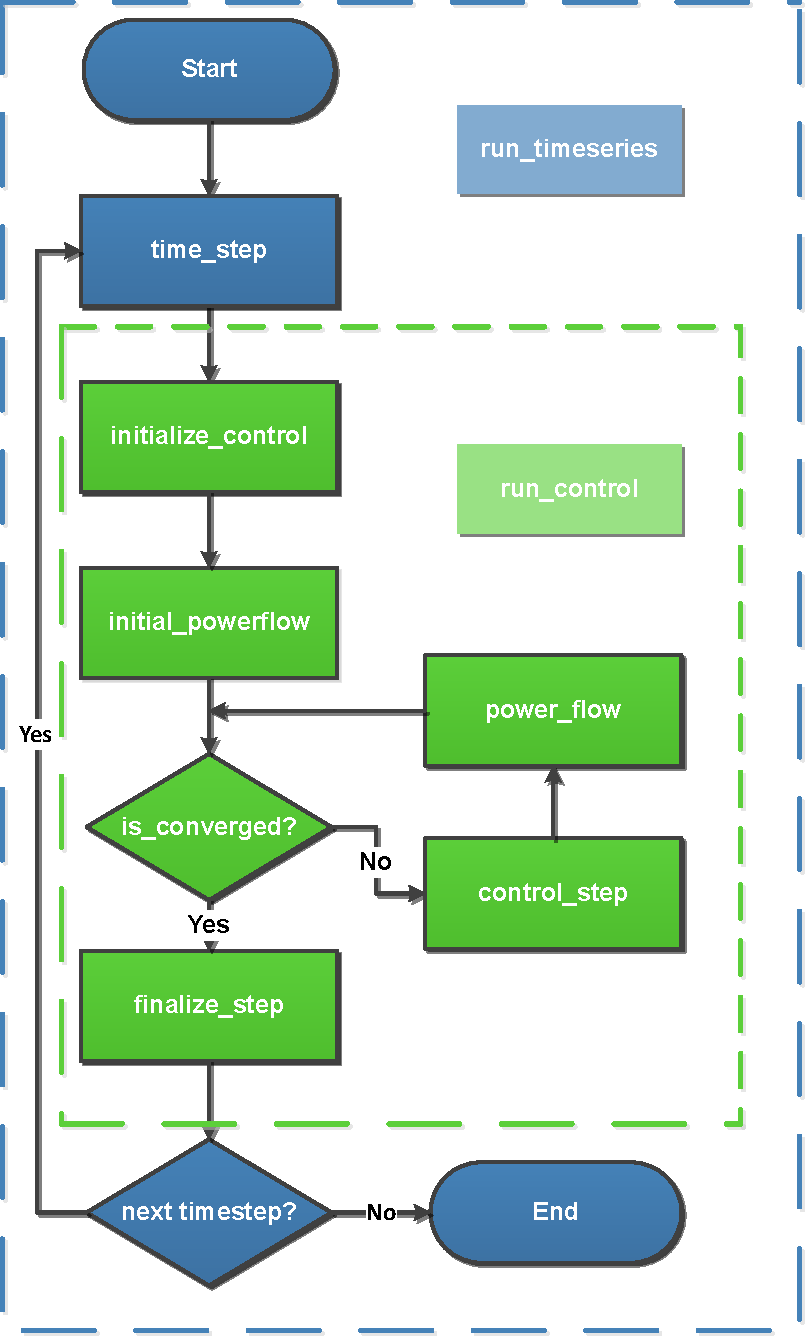
\includegraphics[width=.4\linewidth]{images/Background/Pandapower/run_timeseries_loop.pdf}
% \caption[Pandapower time series calculation]{Pandapower time series calculation loop \cite{pandapowerts}}
% \end{figure}

% After each step, the elements' values are stored in an output writer object and this allows, after the full calculation is finished, to easily save the values on disk.

% \subsection{Other functionality}
% Pandapower has some other features:
% \begin{itemize}
%     \item Predefined Networks. In addition to creating custom networks through the application programming interface (\gls{API}), 66 predefined, published test and benchmark networks can be directly accessed through Pandapower. One of these networks, MV Oberrhein, is the one used in this thesis.
%     \item Plotting features. Pandapower comes with extensive plotting features using the Matplotlib library. All Pandapower elements can be translated into different Matplotlib collections that can be customized with respect to shape, size and colour to allow highlighting and create individual network plots. It is also possible to use colour maps to codify information, like the loading of lines or the voltage at buses.
%     \item Converter. Pandapower includes converters in order to export a Pandapower grid as a MATPOWER or PYPOWER casefile or the other way.
% \end{itemize}



\section{Machine learning overview}
\label{sec:2ml}
%https://www.digitalocean.com/community/tutorials/an-introduction-to-machine-learning
Machine learning is a subset of artificial intelligence that trains a machine to learn. In particular machine learning is the study of how a computer algorithm improves its performances at some task through experience or more precisely:
\begin{quote}
    \centering
    A computer program is said to learn from experience E with respect to some class of tasks T and performance P, if its performance at tasks in T, as measured by P, improves with experience E \cite{mltm}.
\end{quote}
\noindent where generally, in a machine learning problem, T is a task too complex to be solved with human written algorithms.\\

Machine learning differs from the traditional computer science methods.  In traditional approaches, algorithms are sets of explicitly programmed instructions, or rules, used by computers to solve a problem. Machine learning algorithms instead allow computers to train on data inputs and use statistical analysis in order to output values or answers. \\

\begin{figure}[H]
\centering
    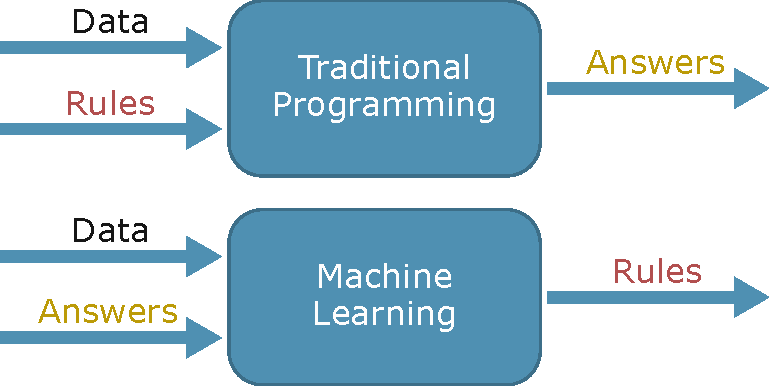
\includegraphics[width=.45\linewidth]{images/Background/ML/MLvstrad.pdf}
\caption[Traditional and machine learning approaches]{Difference between traditional programming and machine learning approach.}
\label{fig:tradvsml}
\end{figure}

\noindent Figure \ref{fig:tradvsml} shows the main difference between traditional methods and machine learning approach: when solving a problem, traditional programming required someone (usually an expert in the field) to generate some rules that would be used to get answers from the input data; while in machine learning the model tries to find some rules that link the input data and the output data (or answers). Machine learning approach has demonstrated to outperform humans in finding this kind of rules, moreover no real expert is required. \\

In machine learning, tasks are classified into some categories. These categories are based on how learning is received or how feedback on the learning is given to the system developed.
There are three main types of machine learning algorithms: supervised, unsupervised and reinforcement learning.\\
This thesis focuses on supervised and reinforcement learning.

% \subsection{History}
% A brief timeline with the most significant achievements in the machine learning field: \\
% in \emph{1943} Walter Pitts and Warren McCulloch published a paper with the first mathematical modelling of a neural network, taking inspiration from the human biology, Pitts thought as human neuron cell as a threshold logic unit working together with other neurons to build a complex system \cite{McCulloch1943}; in \emph{1950} Alan Turing introduce the Turing Test, a method that tests the machine's ability to show human intelligence \cite{turingtest}; in \emph{1952} Arthur Samuel developed a program on an IBM computer that could play checkers and improve over time; in \emph{1956} the Dartmouth College summer AI conference is considered the birthplace of artificial intelligence where McCarthy coins the term for the first time; in \emph{1957} Frank Rosenblatt deigned the first neural network called perceptron \cite{Rosenblatt1958ThePA} which one year later will be tested on computer, achieving good results, it was able to learn to distinguish right punched card form the left punched cards; in \emph{1963} Leonard Uhr and Charles Vossler described the first machine learning algorithm that could adaptively acquire and modify features and thereby overcome the limitations of simple perceptrons of Rosenblatt; in the same year Donald Michie wrote a program that solved the tic-tac-toe game; in \emph{1970} Seppo Linnainmaa published a paper about the reverse mode of automatic differentiation, later this method will be known as back propagation; in \emph{1980} Kunihiko Fukushima published a paper on neocognitron, a hierarchical multilayer \gls{ANN} that can "learn without a teacher", used for patter recognition tasks, such as digits recognition \cite{neocognitron}; in \emph{1982} Hopfield made popular a type of recurrent neural network \cite{hopfield}; in \emph{1989} Chris Watkins introduce Q-learning, a reinforcement learning algorithm that looks for the best action for a given state; in \emph{1992} Gerald Tesauro developed a program capable of playing the game backgammon; in \emph{1995} were published influential papers on random forest and support vector machines; in \emph{1996} IBM's Deep Blue, a chess-playing program beat the chess champion at that time, Garry Kasparov; in \emph{1996} a team led by Yann LeCun released the MNIST dataset which will be widely adopted for handwriting recognition; in \emph{2006} Geoffrey Hinton coined the term "deep learning"; in \emph{2009} Fei-Fei Li published the ImageNet dataset, a large dataset for image recognition; in \emph{2012} Alex Krizhevsky, Ilya Sutskever, Geoffrey Hinton developed the AlexNet neural network that improved the accuracy of image recognition \cite{alexnet}; in \emph{2014} Facebook publish the DeepFace algorithm to identify individual in photos; in \emph{2016} Google's AlphaGo program beat the strongest Go player at that time; \emph{2019} DeepMind's AlphaStar reaches Grandmaster level at StarCraft II, outperforming 99.8 percent of human players.


\subsection{Artificial neural networks}
Nowadays, a popular approach to solve machine learning problems is to use artificial neural networks (\glspl{ANN}), whose main elements are the \emph{neurons}.\\

\gls{ANN} is a computational model that consists of several processing elements that receive inputs and deliver outputs based on their predefined activation functions. They have been proved to provide a strong approach to approximate functions in order to solve continuous and discrete problems. \\

They have been inspired by the biological neural networks that constitute animal brains. For the first time, in \emph{1943} Walter Pitts and Warren McCulloch published a paper with the mathematical modelling of a neural network. They thought a human neuron cell as a threshold logic unit working together with other neurons to build a complex system: a neuron cell collects multiple signals arriving at the dendrites, elaborate them and if the accumulated signal exceeds a certain threshold, an output signal is generated that will be passed on by the axon \cite{McCulloch1943}. So, the idea behind \glspl{ANN} is to link many simple units (neurons) to develop a more complex system (brain).

\begin{figure}[H]
\centering
    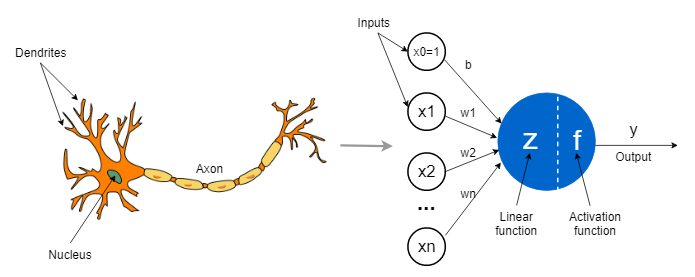
\includegraphics[width=.8\linewidth]{images/Background/ML/Perceptron.png}
\caption[Perceptron representation]{Representation of a biological neuron (left) and its artificial equivalent (right).}
\label{fig:linsep}
\end{figure}

\subsubsection{Perceptron}
\label{sssec:perc}
The simple unit in an \gls{ANN} is called a \emph{perceptron}. The perceptron is a mathematical function that takes some inputs, weights them separately, sums them and pass the sum through a nonlinear function to produce an output. \\
This mathematical function can be written as follows:
\begin{equation} \label{eq:perceptron}
    o(x_1,x_2,...,x_{n-1}, x_n) = f(\sum_{i=0}^n w_i x_i + w_0)
\end{equation}
\noindent where $n$ is the number of connected neurons, $x_i$ is the input from the neuron $i$, $w_i$ is the weight that determines the contribution of input $i$, and $f$ is a nonlinear function. A possible example of the function $f$ is: 
\begin{equation*}
  f(x) =
    \begin{cases}
      1 \, \text{if} \, x > T \\
      -1 \, \text{otherwise}
    \end{cases}       
\end{equation*}
\noindent with $T$ a real value representing the threshold that $x$ has to surpass for the function to output $1$. In the formula \ref{eq:perceptron} the threshold $T$ is given by the value $w_0$. \\

A single perceptron can be used for binary classification tasks: it builds a hyperplane that separates the data, and outputs giving a value between -1 and 1 whether a point is on a side of the hyperplane or on the other side. The perceptron can find a hyperplane in any n-dimensional space as long as this decision boundary exists; this happens if the data points are \emph{linearly separable}.

\begin{figure}[H]
\centering
    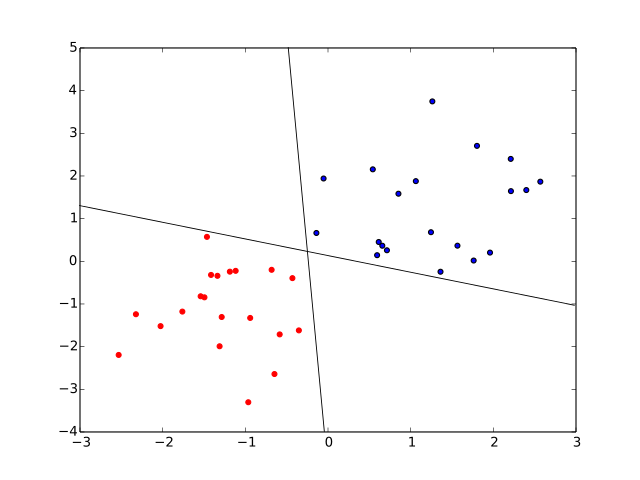
\includegraphics[width=.6\linewidth]{images/Background/ML/Perceptron_cant_choose.svg.png}
\caption[Linearly separable data]{Example of linearly separable data. The two lines are some possible representations of hyperplanes that divide the data \cite{linsep}.}
\label{fig:linsep}
\end{figure}

The weights' values are generally initialised randomly, and their values are changed during training using the \emph{perceptron training rule} where each weight $w_i$ in $\textbf{w}$ is changed according to:
\begin{equation} \label{eq:percrule}
    \begin{aligned}
        \textbf{w} = \textbf{w} + \Delta \textbf{w}\\
        \Delta \textbf{w} = \alpha (\textbf{t}-\textbf{o})\textbf{x}
    \end{aligned}
\end{equation}
\noindent where $\textbf{x}$ are the inputs, $\textbf{o}$ the outputs of the perceptron, $\textbf{t}$ the target outputs and $\alpha$ is a scaling factor called learning rate, used to reduce the change of the weights $\textbf{w}$ at each step. Equation \ref{eq:percrule} assures convergence under the specific condition of the linearly separable training samples.\\

A better training rule is the \emph{delta rule} that uses the \emph{gradient descent} to find the weights that best fit the training examples. This training rule requires the definition of a loss function $L$ that has to be differentiable.\\
This loss function is used to calculate the derivative of the loss \gls{wrt} to the weights:
\begin{equation} \label{eq:chainrule}
    \nabla L(\textbf{w}) = \Big[ 
                \frac{\partial L}{\partial w_0},
                \frac{\partial L}{\partial w_1},
                \cdots,
                \frac{\partial L}{\partial w_{n-1}},
                \frac{\partial L}{\partial w_n}
                        \Big]
\end{equation}
\noindent where $\nabla L(\textbf{w})$ is the gradient of $L$ \gls{wrt} the weights $\textbf{w}$. Geometrically, $\nabla L(\textbf{w})$ is a vector in the weights' space that represents the steepest increase in $L$. So, the formula \ref{eq:percrule} is updated as follows:
\begin{equation*}
    \begin{aligned}
        \textbf{w} = \textbf{w} + \Delta \textbf{w}\\
        \Delta \textbf{w} = -\alpha \nable L(\textbf{w})
    \end{aligned}
\end{equation*}
\noindent where $\alpha$ is the learning rate and the minus sign is used to move towards the direction that \emph{minimise} the loss $L$.\\

This gradient descent rule is the base of the backpropagation algorithm commonly used when training deep artificial neural networks.\\

Perceptrons are the basis for more complex models like for example: multi layer perceptrons, convolutional neural networks and recurrent neural networks.

\section{Supervised learning}
\label{sec:sl}
%https://citeseerx.ist.psu.edu/viewdoc/download?doi=10.1.1.457.4869&rep=rep1&type=pdf
In supervised learning, the goal is to learn a function that maps an input $X$ to an output $Y$ based on example input-output pairs and applying this learnt function to predict the output of future unseen data.

\subsection{Formal definition}
\label{ssec:formdefSL}

In a supervised learning problem, the goal is to find a function $f : X \rightarrow Y$, from a sample data $S_n$ composed by pairs of (input, output) points:
\[
S_n = ((x_1,y_1),\dots(x_n,y_n)) \in (X \times Y)^n
\]
Typically, $x_i \subset R^n$ and $y_i \subset R$ for regression problems or $y_i$ discrete for classification problems, for example $y_i \in \{-1,1\}$ for binary problems. \\

In the statistical learning settings, an important hypothesis is that the training data is independently and identically distributed (\gls{iid}) from a probability distribution function $P(X,Y)$. The term \gls{iid} means that the random samples are chosen: \emph{independently}, the samples are considered as independent events, having the value of one sample does not give information about the other samples; and \emph{identically distributed} so the probability of choosing one sample or another is the same, all the samples are equally likely to be chosen.\\ The goal of the learning is to find a mapping function $f$ that can encode the property of $P(X,Y)$ between the inputs X and the output Y. \\

Another important concept is to evaluate how well the function $f$ performs, calculating the error or loss between the predicted values $f(x)$ and the actual value y. This error is evaluated with a loss, or cost, function $L: Y \times Y \rightarrow R^+$. There are many loss functions depending on the problem and requirements, one example is the mean absolute error (\gls{MAE}) loss function:
\[
L(f(x),y)= \frac{1}{N} \sum_{i=0}^{N} |f(x_i)-y_i| 
\]
Many supervised learning algorithms consider the minimisation
of this loss function as an optimisation problem to find the best predictor among all the possible candidate input-output mappings in the solution space $\mathcal{B}$. \\

With the loss function $L(x,y)$, the definition of risk of the function $f$, also called generalisation error, must be introduced:
\[
R(f) = \int L(f(x),y)) \; dP(x,y). 
\]
The objective is to find the function $f$ in $\mathcal{B}$ that minimises the generalisation error, $R(f)$. Since it is not possible to solve $R(f)$, because of the joint probability distribution $P(x,y)$ is unknown, $f$ inferred from available data set $S_n$.\\

Given this loss, a way to minimise it, especially with \gls{ANN} is calculation the gradient of the loss \gls{wrt} the weights and then back propagate the gradient to change the weights' value.

\subsection{Models}
\label{ssec:modelsSL}
In this section is reported the main \glspl{ANN} used for the forecasting part where the models are trained under a supervised learning framework. 

\subsubsection{Multi layer perceptron}
As mentioned in \ref{sssec:perc}, perceptrons can express only linear decision boundaries. To solve this problem, it is possible to use more perceptrons to represent more complex decision surfaces. \\

Multi layer perceptron (\gls{MLP}) networks are constructed by many perceptrons. These perceptrons are organised in layers: there are always at least two layers, input and output layer, and one or more hidden layers; from here the term \emph{multi} layer perceptron. Each layer is composed by many neurons and each neuron in one layer is connected to all the neurons in the next layer, so the information from the input layer is propagated to hidden layers and then to the output layer. These models are also known as deep neural networks (\glspl{DNN}) since the  networks' hidden layers make the models "deep". The output of a layer, before being propagated to the next layer, passes through a non-linear activation function, for example the Rectified Linear Unit (\gls{Relu}), the Sigmoid function or the hyperbolic tangent function (\gls{Tanh}). The non-linearity of the activation function is needed since it introduces more complexity to the model; summing operations of many linear layers is still a linear operation, so, in such case, a deep network would perform similarly to a single layer network.\\

The main idea behind stacking many layers is that each layer represents a boundary region, that it will pass to another layer to represent an even more complex boundary region. Using many layers, it is possible to represent very complex decision boundaries. This sequence of operations can be written as follows:
\begin{equation}\label{eq:chain}
f(x) = f^{(n)}( f^{(...)}( f^{(1)}(x)) )
\end{equation}
\noindent where n is the number of hidden layers, $f^{(n)}(x)$ is the boundary representation at the last hidden layer before the output layer, $f^{(1)}(x)$ is the decision boundary representation at the first hidden layer after the input layer. The result composition of all these functions, $f(x)$, is the mapping function that can solve the requested problem. Equation \ref{eq:chain} can be viewed as a chain, where the output of the first decision boundary is propagated to the next decision boundary function up to the final hidden layer and then to the output layer to get the predictions. This propagation is known as \emph{forward propagation}.\\

The weights in a \gls{MLP} are updated with formula \ref{eq:chainrule}. This process in called backpropagation, since the after calculation of the loss, the gradient of the loss \gls{wrt} each weight is propagated back through all layers.

\subsubsection{Convolutional neural network}
Convolutional neural networks (\glspl{CNN}) are a particular type of \gls{ANN} that process data with a grid-like topology. These kinds of networks are usually used with images, considering an image as a 2D matrix of pixels or for with time series, considering a time series as a 1D structure. \\

% Like artificial neural networks in general, they are an example of brain-inspired ideas coming through an interaction with computer science and engineering
The term convolutional comes from the usage of a mathematical operation called convolution. Convolution is a linear operation that involves two functions (or matrices in the discrete case), $x$ and $w$:
\begin{equation}
    (x \ast w)(t) \overset{def}{=} \int_{-\infty}^{\infty} x(\tau) \cdot w(t-\tau) d\tau
\end{equation}
\noindent where $\ast$ is the sign for the convolution and $\cdot$ is the sign for the dot product.\\
The output of this linear operation, given by the input $x$ and the weights $w$ (also called \textbf{kernel} or \textbf{filter}) is referred to as \textbf{feature map}. \\

% There are three main operations in a convolutional layer: \textbf{convolution}, \textbf{activation function} and \textbf{pooling function}. 

The main idea is to \emph{convolve} the input, for example an image, with a filter of size $f$. The filter is applied to an area of the image, and the dot product between the that portion of the input image and the filter is computed. Then the filter is shifted to the next portion of the input image, and this way the dot product is calculated for the full width and height of the input.\\
Since the convolution is a linear operation, the output of the convolution must go through a non-linear activation function, usually \gls{Relu} in the case of \glspl{CNN}. \\

The output of a convolutional layer is passed to a pooling function. This pooling function aggregates the output of the convolutional layer at a certain location with a number that statistically represents their values. This allows to reduce the data dimensionality, to shorten the training time and to reduce overfitting.\\
Usually, the most common pooling function are max pooling, which takes the max value of the window, or average pooling, which averages the values of the window. \\

With these series of operation, a single convolutional block can extract some important features from the input data. Generally, many convolutional blocks are stacked together so that each of the next block can represent more complex and specific features. \\
The output of the last block is flatten and passed to one or more fully connected layers to get the final prediction (in case of a classification task). \\

\begin{figure}[H]
\centering
    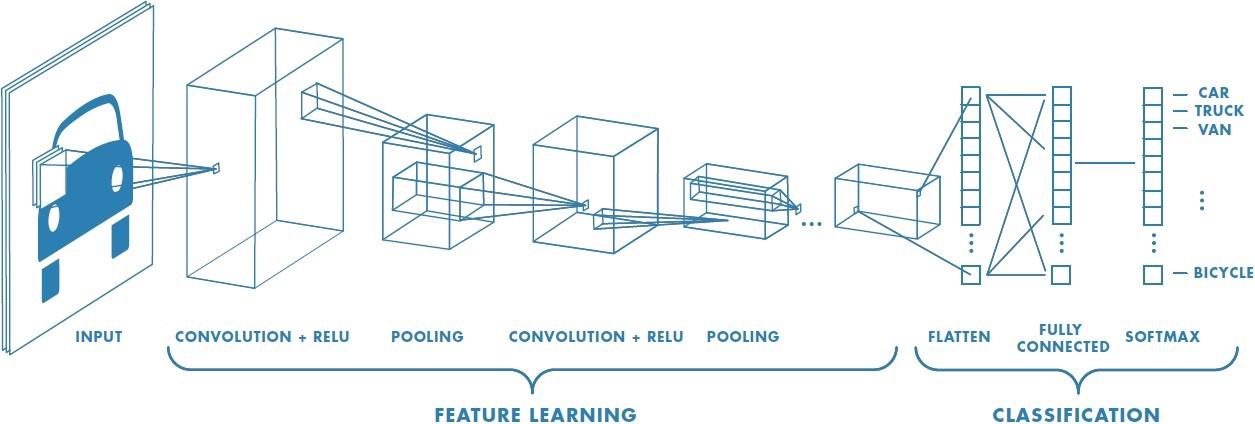
\includegraphics[width=.75\linewidth]{images/Background/ML/ConvNNjpeg.jpeg}
\caption[Graph representation of a convolution neural network]{Graph representation of a \gls{CNN}. It is possible to notice some convolutional and pooling layers (left) and the final fully connected layer (right) \cite{cnn}.}
\end{figure}

\glspl{CNN} have shown to perform very well on some task, especially image classification, and their main advantages are lower number of  weights compared with a \gls{MLP} network and the ability to automatically learn how to extract important features.

\subsubsection{Recurrent neural network}
Recurrent neural networks (\glspl{RNN}) are a particular type of \gls{ANN} that work well with time series data or data that can be represented as a sequence. \glspl{RNN} use the output of the network units at time $t$ as the input of the other units at time $t+1$. \\

Generally, \glspl{RNN} are represented as follows:\\

\begin{figure}[H]
\centering
    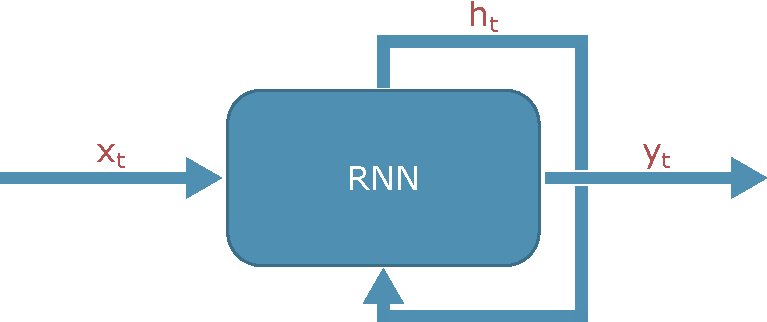
\includegraphics[width=.55\linewidth]{images/Background/ML/RNN.pdf}
\caption[Graph representation of a recurrent neural network]{Graph representation of a \gls{RNN}.}
\end{figure}

\noindent where x is the input, the \gls{RNN} rectangle is the recurrent network block and y is the output of the model. The arrow coming out and back in the RNN block is what the term \emph{recurrent} refers to: after receiving an input, at time $x_t$ the RNN computes some operation and a hidden state, $h_t$, is saved and used for the next input, at time $t+1$.  \\

Mathematically, this process can be represented with the following formula:
\begin{equation*}
    h_t = f_W(h_{t-1},x_t)
\end{equation*}
\noindent where $f_W$ is a function that takes as input the hidden state of the previous time step $h_{t-1}$ and the input at the current time step $x_t$ and it outputs the hidden state at the current time step $h_t$. At the next time step $t+1$, the previous hidden state $h_t$ would be passed with the next input $x_{t+1}$ to $f_W$ and so on until all the input time steps are consumed.\\

An important concept to notice is that the function $f_W$ depends on some weights $W$, and these weights are shared for every time step of the computation. For example, the function $f_W$ can be represented as:
\begin{equation*}
    f_W = Tanh(W_h \cdot h_{t-1} + W_x \cdot x_{t})
\end{equation*}
\noindent where \gls{Tanh} is the hyperbolic tangent function, $W_h$ is the matrix of weights that multiplies the hidden state $h_{t-1}$ and $W_x$ is the matrix of weights that multiplies the hidden state $x_{t}$. \\

% \subsubsection{Long Short-Term Memory networks}
\noindent\textbf{Long Short-Term Memory networks}\\

\noindent A popular problem with \gls{RNN} networks is exploding or vanishing gradient. Due to the recurrent nature of the model, during backpropagation, the partial derivatives generate chains of matrix multiplications. In case of large derivates, the gradient increases exponentially, resulting in too large values to be handled by a calculator; this is often referred to as \emph{exploding gradient}. In the opposite case, if the gradient is small, the gradient decreases and the model would stop learning; this is often referred to as \emph{vanishing gradient}.\\

A model that can solve these gradient problems is the Long Short-Term Memory (\gls{LSTM}) networks. They were designed to handle the long-time dependency of the input. The main difference between a simple \gls{RNN} and a \gls{LSTM} network is the complexity of the hidden block: while in a \gls{RNN} there is only a \gls{Tanh} function, in a \gls{LSTM} there usually is the \gls{Tanh} function and as well some Sigmoid functions. \\
This more complex model allows the network to keep in memory (as a hidden state) or forget some information that are considered as not too relevant \cite{lstm}.

\subsection{Evaluation metrics}
\label{ssec:evalmetricSL}
An important part of a machine learning problem is to evaluate whether a model performs well or not. There are many ways to evaluate a model, these are commonly referred to as evaluation metrics.\\

The evaluation metrics differ from task to task. There are many specific evaluation metrics for classification problems. Some of the most common are presented in this section.\\

Some terms have to be introduced. During classification, there are four outcomes that can occur:
\begin{itemize}
    \item \textbf{True positive (\gls{TP})}: when the result of a test tells that a subject belongs to a particular class (its result is positive), and it actually belongs to that class (the result is true, correct).
    \item \textbf{False negative (\gls{FN})}: when the result of a test tells that a subject does not belong to a particular class (its result is negative), but it actually belongs to that class (the result is false, wrong).
    \item \textbf{True negative (\gls{TN})}: when the result of a test tells that a subject does not belong to a particular class, and it actually does not belong to that class.
    \item \textbf{False positive (\gls{FP})}: when the result of a test tells that a subject belongs to a particular class, but it actually does not belong to that class.
\end{itemize}
% These different outcomes can be represented in a confusion matrix. \\

% \emph{add confusion matrix image} \\

When a test is wrong (either \gls{FP} or \gls{FN}) a misclassification occurs. The evaluation metrics try to quantify how well a model performs, elaborating how many miss classifications were done.

\subsubsection{Accuracy}
Accuracy measures how often the model classifies correctly. Accuracy is defined as the ratio between the number of correct classifications and the total number of predictions.
\[
accuracy = \frac{\text{correct predictions}}{\text{total predictions}} = \frac{TP + TN}{TP + TN + FP + FN}
\]
\subsubsection{Recall}
Recall, also called sensitivity or true positive rate, gives the proportion of positive cases correctly identified by the tests. Recall is defined as the ratio between the positive subjects correctly identified and the total number of positive subjects.
\[
recall = \frac{TP}{TP + FN}
\]
\subsubsection{Precision}
Precision gives the proportion of correct positive tests and the number of all tests whose result was positive.\\
% Precision explains the proportion of subject actually belonging to a class and the number of tests that attributes the subjects to that specific class. 
Precision is defined as the number of true positives divided by the number of predicted positives.
\[
precision = \frac{TP}{TP + FP}
\]
\subsubsection{Trade-off recall precision}
Generally there must be a trade-off between recall and precision, or equivalently between the number of false negative and false positive, since increasing the recall (precision) would decrease the precision (recall). \\

This trade-off is even more important when a misclassification would be worse than the other: predicting a subject to have an illness, but actually it is sane (\gls{FP}) or predicting a subject sane, but actually it has an illness (\gls{FN}). In this medical case, \gls{FN} would be a worse case, since the illness of the subject would not be treated while \gls{FP} would have only to take some medications. \\
In general, the trade-off depends on the task and there is not a specific way to tell a priori if \gls{FP} is a better case than \gls{FN}.

\subsubsection{F1-score}
There are other situations where having \gls{FP} or \gls{FN} does not change much, they are equally important.\\
In these cases, it is often convenient to combine recall and precision in a single evaluation metric. It is defined by the harmonic average of the recall and precision.
\[
F1\!-\!score = 2\cdot \frac{precision \cdot recall}{precision + recall}
\]

% \subsubsection{Average Return}
% For what concerns the evaluation of \gls{RL} models, there are not standard metric to 

\subsection{Unbalanced dataset}
\label{ssec:unbalan}
Unbalanced datasets are common in real life classification problem. An unbalanced dataset is a dataset where a class is unrepresented \gls{wrt} the other classes; so the classes' distribution is not even. As it usually happens, the observations in the minority class are the most important and the problem is more sensitive to misclassification of that class: fraud detection, for example.\\

Generally this is a difficult problem since some models may not generalise well: the model receiving more observation of a class tends to be more biased towards it and fails to understand the patters that separate the classes. \\
In these cases, it is also important to consider which evaluation metric to use. Accuracy metric, in general, is not a meaningful metric, since the model predicting every observation as belonging to the over-represented class would get a high score. More meaningful metrics are precision, recall or an average of the two, for example F1-score.\\

There are few methods to solve or mitigate the unbalanced dataset issue. Some of them will be reported here:
\begin{itemize}
    \item Resample the dataset: this can be done, increasing the number of observations in the minority class (\emph{oversampling}) or decreasing the observation in the majority class (\emph{undersampling}). \\
    The two main methods to resample the dataset are described in the following part:
        \begin{itemize}
            \item Undersampling: the main idea is to reduce the number of instances in the majority class to the underrepresented class' level. \\
            This is usually done with a random downsampling, randomly discarding samples.\\
            
            A possible problem with this technique is that it does not care to discriminate importance that the different observations may have.\\
            
            There are some other more informative techniques like for example nearest neighbours algorithms that try to include samples from every cluster in the majority class.
            \begin{figure}[H]
                \centering                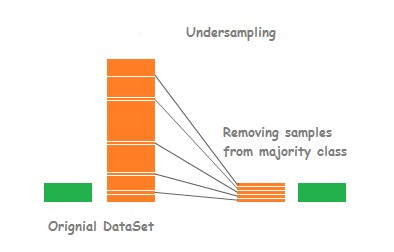
\includegraphics[width=0.55\linewidth]{images/Background/Unbalanced/Undersampling.jpg}
                \caption[Undersampling technique]{Undersampling technique \cite{unbalanced}.}
                % \label{fig:MVober}
            \end{figure}
            
            \item Oversampling: opposite to undersampling, its main idea is to increase the number of instances in the minority class. \\
            This is usually done generating synthetically observation of the underrepresented class base on the available data. \\
            Some popular techniques include Variational Autoencoders (VAE), \gls{SMOTE} (Synthetic Minority Oversampling Technique) or MSMOTE (Modified Synthetic Minority Oversampling Technique).
            \begin{figure}[H]
                \centering                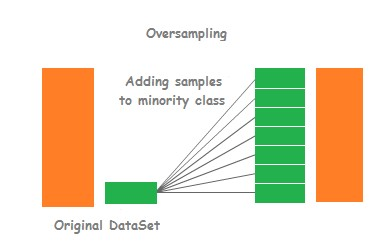
\includegraphics[width=0.55\linewidth]{images/Background/Unbalanced/Oversampling.jpg}
                \caption[Oversampling technique]{Oversampling technique \cite{unbalanced}.}
                % \label{fig:MVober}
            \end{figure}
            In this thesis, the method \gls{SMOTE} will be used. \gls{SMOTE} generates synthetic samples of the minority class. The main idea is to find examples that are close in the feature space, draw a line between them, and then a new sample is chosen on that line. In particular, a random sample from the minority class is chosen, some other k samples are chosen close to it (usually k=5, and they are chosen using k nearest neighbor algorithm), among these k, one is selected randomly, and then a synthetic element is created on the line that links the two selected samples.
        \end{itemize}
    \item Penalise misclassification: the idea is to penalise misclassification of the minority class more than the majority class. In this way the model should put more focus on the underrepresented observation since a penalty in case of error is larger than the major class error. \\
    These penalties are commonly referred to as weights, and finding the right weights' values is usually challenging.
    Commonly, the weights are calculated as follows:
    \[
        w_i = \frac{total\_samples}{num\_classes \cdot num\_samples_i}
    \]
    \noindent where $w_i$ is the weight for class $i$, $total\_samples$ is the number of total samples available, $num\_classes$ is the number of unique classes (2 in a binary classification task), $num\_samples_i$ is the number of sample belonging to class $i$.
\end{itemize}



\section{Reinforcement learning}
\label{sec:rl}
Reinforcement Learning (\gls{RL}) is a machine learning technique that tries to solve a problem in which a decision-maker, agent, can perform some actions inside a world, called environment. The agent senses the environment through the state and for each state the agent has to perform an action. These actions have two results: they change the agent's state and give him a feedback, the reward. The reward is a value which indicates if the action performed is good, then the reward is positive, or it is bad, the reward is negative. Given these rewards, the agent understands what action to perform in a given state to get a positive reward. This cycle of state-action-reward is repeated many times. The goal of the agent is to find a policy such that the actions performed lead to the maximum reward possible.\\

\glg{RL} has become popular in the last years thanks to results obtained in some game environment like, Backgammon (\cite{rlback}), Atari games (\cite{rlatari}), Go (\cite{rlgo}) but also robotics (\cite{rlrob}), self-driving cars, finance and other fields (\cite{rlappl})


\subsection{Formal definition}
\label{ssec:formdefRL}
Reinforcement learning can be formulated as a Markov decision process (\gls{MDP}), indeed a \gls{MDP} express the problem of sequential decision-making, where for each state $s$, the decision maker can choose any action $a$ available in that state $s$. The process responds by moving with some probability to the state $s^\prime$ and giving the decision maker a reward $R_a(s,s^\prime)$. %(read as: `the reward given when in state $s$ and the action $a$ chosen brings to the next state $s^\prime$')
\\
The \gls{MDP} is defined as a tuple of 4 elements (S, A, P, R), where:
\begin{itemize}
\item S is a set of states, called the \emph{state space}.
\item A is a set of actions, called the \emph{action space}.
\item P is the probability from state $s$, at time $t$, of reaching state $s^\prime$, at time $t+1$ with action $a$:
\[P_a(s,s^\prime) = Pr(s_{t+1} = s^\prime | s_t = s, a_t = a)\]
\item $R_a(s,s^\prime)$ is the immediate reward received after transitioning from state $s$ s to state $s^\prime$, due to action $a$; so the reward at time $t$, also $r_t$.
\end{itemize}
The state and action space may be finite or infinite.\\

The \gls{MDP} is controlled by a sequence of discrete time steps that create a trajectory $\upsilon$:
\[s_0 \xrightarrow{a_0} s_1 \xrightarrow{a_1} s_2 \xrightarrow{a_2} s_3 \xrightarrow{a_3} \dotso\]
where the states follow the state transition $P_a(s,s^\prime)$. The transition function and the reward function are determined only by the current state, and not from the previous states. This property is called Markov property, which characterises the MDP and it means that the process is memoryless and that the future state depends only on the current one and not on its history. 


The goal of the \gls{MDP} is to find a good policy for the decision maker, that is, a function $\pi$ that specifies the action $a$ that will be chosen when in state $s$. The policy $\pi$ found will maximise the cumulative reward over a trajectory $\upsilon$:
\[ G(\upsilon) = \sum_{t=0}^{\infty} r_t \] 
%R_{a_0}(s_0, s_{1}) + R_{a_1}(s_1, s_{2}) + \dotso =
This return value has the problem that all the rewards contribute in the same weight and this can create some problems due to the lack of temporal information. A better return value would be to give more importance to the short-term memories and giving less importance to the ones far in the future. This is solved by introducing a discount factor, denoted with $\gamma$. Then the corrected formula is: 
\[ G(\upsilon) = \sum_{t=0}^{\infty} \gamma^t r_t \]
with value of $\gamma$ satisfying $ 0 \leq \gamma \leq 1$. When $\gamma$ is closer to zero, the agent will tend to consider only immediate rewards whether if $\gamma$ is closer to one, the agent will consider future rewards with greater weight, willing to delay the instant reward in favour of a greater cumulative reward. 
This new definition of $G(\upsilon)$ is the total discounted reward.

A simple decomposition of $G(\upsilon)$ is : 
\[ G_t(\upsilon) = r_t + \gamma G_{t+1}(\upsilon)\]
so the return value $G$ can be divided in the reward at time $t$ plus the discounted total reward at time $t+1$.


%http://incompleteideas.net/book/ebook/node34.html
%https://cims.nyu.edu/~donev/Teaching/WrittenOral/Projects/XintianHan-WrittenAndOral.pdf
Another important notion in \gls{MDP} and \gls{RL} is the value function, known as V-function. While the return $G(\upsilon)$ gives the reward over a trajectory, it does not tell much about how good the single states are. The value function does exactly this: it estimates how good it is for the decision maker to be in a given state. The notion of "how good" is defined in terms of future rewards that the decision maker can expect in terms of expected return.
\\
The value function $V_{\pi}(s)$ can be formally defined as: 
\[V_{\pi}(s) = \mathbb{E}_{\pi}(G(\upsilon)|s_0=s) = \mathbb{E}_{\pi}(\sum_{t=0}^{\infty} \gamma^t r_t|s_0=s)\]
\vspace{-9.3mm}
\begin{center}
The expected return when starting at state $s$ and following policy $\pi$.
\end{center}

\noindent Similarly, it is possible to define the action-value function, also known as Q-function as the expected return from state $s$ with an initial action $a$:
\[Q_{\pi}(s,a) = \mathbb{E}_{\pi}(G(\upsilon)|s_0=s, a_0=a) = \mathbb{E}_{\pi}(\sum_{t=0}^{\infty} \gamma^t r_t|s_0=s,a_0=a)\]

Furthermore, the value function and the action-value function are related and satisfy a particular relationship, used in many \gls{RL} contests, that for any policy $\pi$ and state $s$, the following condition holds:
\[V_{\pi}(s) = \mathbb{E}_{\pi}(Q_{\pi}(s,a))\]

Knowing the optimal Q-function ($Q^\star$), to maximise the V-function ($V^\star$), the action best has to be found. This is found with:
\begin{equation} \label{eq:besta}
    a^\star(s) = argmax_a Q^\star(s,a)
\end{equation} 
That is: the best action is the one that maximises the Q-function.
\pp
Moreover, the V-function can be decomposed in two terms:
\begin{equation} \label{eq:bl}
V_{\pi}(s) = \mathbb{E}_{\pi}(G(\upsilon)|s_0=s) =
					\mathbb{E}_{\pi}( r_t + \gamma V_{\pi}(s_{t+1})|s_t=s)
\end{equation}
\begin{center}
where $r_t$ is the reward at time $t$ and $\gamma V_{\pi}(s_{t+1})$ \\the discounted total reward of the next state.
\end{center}

\noindent The equation in \ref{eq:bl} is the Bellman Equation that defines the value function recursively, enabling the estimations of the next states. \\
Similarly, it is possible to write the Bellman equation for the Q-function:
%(using the V-function and Q-function relationship)
\[Q_{\pi}(s,a) = \mathbb{E}_{\pi}(G(\upsilon)|s_0=s, a_0=a) = 
\mathbb{E}_{\pi}(r_t + \gamma Q_{\pi}(s_{t+1},a_{t+1})| s_t=s, a_t=a) \]
In this way the V-function and the  Q-function are updated with the values of the successive states without the need to know the trajectory till the end.


\subsection{Model}
\label{ssec:modelsRL}
In this section is being reported the main \glspl{ANN} used for the controlling part. 

\subsubsection{Deep deterministic policy gradient}
\label{sssec:ddpg}
As state in equation \ref{eq:besta}, it is possible to see that the best action is chosen in order to maximise the Q-function among all the possible actions.\\
This works in the case of a discrete action space, where it is possible to easily compute the $argmax_a$ operation, just comparing the Q-values of each action. This is not obvious for a continuous case.\\

The deterministic policy gradient (\gls{DPG}) implementation tries to solve this problem. The idea behind \gls{DPG} is to learn a deterministic function $\mu_{\phi}(s)$ that can approximate the $argmax_a Q(s,a)$ operation.\\
One possible way to find this deterministic function is using \gls{ANN} and in particular deep neural networks. So, the term deep deterministic policy gradient merges the \gls{DPG} idea with the use of \gls{ANN}. \\

In particular, the \gls{DDPG} is an actor-critic algorithm, and it uses two neural networks. The actor (characterised by weight parameters $\phi$) decides the action to perform in a given state, and the critic (characterised by weight parameters $\theta$) evaluates the action chosen by the actor.

\begin{figure}[H]
\centering
    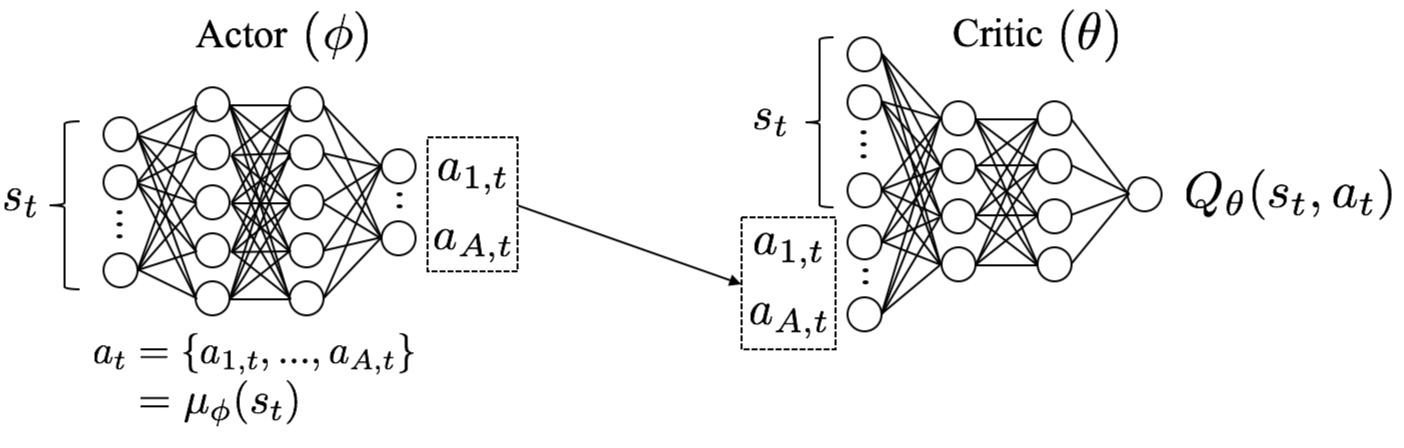
\includegraphics[width=1\linewidth]{images/Background/RL/DDPG archi.PNG}
\caption[DDPG architecture]{Actor-critic model architecture of the \gls{DDPG} agent \cite{DDPGvc}.}
% \label{fig:MVober}
\end{figure}

\noindent During exploration, give the state $s_t$ the agent performs some action $a_t$, moving to the next state $s_{t+1}$, obtaining a reward $r_t$. This information, with a boolean flag stating if the game ended ($d_t$) or not, is stored in a replay memory as a tuple $(s_t,a_t,r_t,s_{t+1},d_t)$. This replay memory is then used during training: a batch $B$ is randomly chosen, and the agent is trained on it.\\ %This batch is used to get the Q-values.\\
Both networks are trained, updating the weights $\phi$ and $\theta$, in particular, the weight from the critic are update with gradient descent and following loss:
\begin{equation} \label{eq:losscritic}
    \mathcal{L}(\theta) = \sum_B \Bigg( \underbrace{Q_{\theta}(s_t,a_t)}_{i} - \Big( \underbrace{r_t + (1-d_t)\gamma Q_{\theta}\big(s_{t+1}, \mu_{\phi}(s_{t+1})\big) }_{ii} \Big) \Bigg)^2
\end{equation}

\noindent At the same time, the actor network's weights $\phi$ are updated maximising the following loss function with gradient ascent:
\begin{equation} \label{eq:lossactor}
    \mathcal{L}(\phi) = \sum_B Q_{\theta}\big(s_t,\mu_{\phi}(s_t)\big)
\end{equation}
The goal is to update the weights such that the action chosen by the actor ($\mu_{\phi}(s_t)$) maximises the Q-value ($Q_{\theta}(s_t,a_t)$).\\

Given equation \ref{eq:losscritic} it is possible to see that both the predicted value $i$ and the target value $ii$ are calculated with the same network $Q_{\theta}$, this makes the training unstable. A solution to this problem is to use two other target networks $\phi_{target}$ and $\theta_{target}$. So the equation \ref{eq:losscritic} becomes:
\begin{equation*} \label{eq:losscritic2}
    \mathcal{L}(\theta) = \sum_B \Bigg( Q_{\theta}(s_t,a_t) - \Big( r_t + (1-d_t)\gamma Q_{\theta_{target}}\big(s_{t+1}, \mu_{\phi_{target}}(s_{t+1})\big)  \Big) \Bigg)^2
\end{equation*}

\noindent While the equation \ref{eq:lossactor} does not change.\\

The target networks weights are updated after a fixed number of steps, suing the Polyak averaging:
\begin{equation} \label{eq:polyak}
     \phi_{target} = \rho\phi + (1-\rho) \phi_{target}
\end{equation}

\noindent where $\rho$ is a scaling factor usually very small.\\
In a similar way, equation \ref{eq:polyak} is used when updating the critic target network.


\subsection{Evaluation metrics}
\label{ssec:evalmetricRL}
Generally, the evaluation metrics for \gls{RL} are different from the ones of supervised learning. \\
Moreover, in a \gls{RL} framework there are no standard metrics, but it depends on the task that it is trying to solve.\\

A popular evaluation of the agent's choices is looking at the reward over each step, or the cumulative reward over each episode. If the agent is learning well, the reward will increase over time.\\
% So a plot of the agent's reward is reported during the training\\

For this specific task some other statistics about the agent performance are reported, in particular 
an analysis of when the agent choses an action is reported in the results chapter. These statistics refer to the usage of the active and reactive power and if the action chosen was needed to solve the critical voltage situation or not.

\section{Literature review}
\label{sec:lr}
The interest in power networks has increased in the last years, especially for the introduction of distributed energy resources and the progress in the field of artificial intelligence. Particular attention is paid to the dispatching of the required power, as it is important for a utility company to predict the load consumed in order to avoid losses. Predicting the power demand is important because the energy generation must balance the consumption, since there are no efficient ways to store the surplus energy at a reasonable cost. Some papers have tried to forecast the load requests with different techniques: support vector machine \cite{lr_svmload}, wavelet transform \cite{lr_wavt}, some exponential smoothing methods \cite{lr_expsmo}, artificial neural network \cite{lr_annload}. The authors in \cite{lr_rnnload} use an interesting approach with a recurrent gradient boosting regression model to predict the future load consumption and detect power theft. Similarly, some papers deal with the forecasting of the wind generators' output using radial basis function \cite{lr_rbfgen}, support vector machine \cite{lr_svmgen} and recurrent neural network \cite{lr_rnngen}.\\
A lot of concern is placed in forecasting devices' critical situations in the network. The authors in \cite{lr_godm} perform a deep analysis of a network using classification methods to predict critical loading situations and regression models to predict the bus voltage magnitudes; the tests are limited to only multi layer perceptron as deep models. The authors in \cite{lr_frnn} predict the over voltage instabilities using a recurrent neural network in a low voltage distribution network. The authors forecast buses critical situations considering the voltage's phase angles information of consecutive buses instead of the voltage magnitudes; the tests are limited to a small network and time series are not taken in consideration. In \cite{lr_fblack}, authors perform voltage security monitoring, with particular attention to blackouts, using different machine learning models; among which multi layer perceptron models.\\
Some possible ways are proposed to reduce the number of contingencies in the power networks. The authors in \cite{lr_copf} use optimal power flow calculation to control generators' active and reactive power in a small distribution network, in \cite{lr_cdb} the authors propose a droop-based reactive power compensation.\\ Thanks to its increasing popularity in many fields; when solving voltage problems, some solutions have been proposed with reinforcement learning algorithms: in \cite{gym-anm} the authors developed some reinforcement learning environment playgrounds where they tested proximal policy optimisation and soft actor-critic algorithms; in \cite{lr_csi} the authors used a deep deterministic policy gradient algorithm to change active and reactive power of the generators; in \cite{lr_cmadarl} authors used multi deep reinforcement learning framework to control static var compensators and batteries to balance the voltage magnitude in a network; for a similar task, the same authors, in \cite{lr_cfiq} control generators' reactive power; in \cite{lr_fremi} authors control batteries and heat pumps to maximise energy consumption and reduce losses.\\
The mentioned works either: \emph{a)} consider only small test networks, \emph{b)} do not deal with unbalanced datasets, and \emph{c)} have high values of active curtailment. These are some limitations since: \emph{a)} small networks may result in a not realistic analysis, \emph{b)} power grids are highly secure, so the number of voltage problems is small with respect to the number of non-critical situations, \emph{c)} the goal is to minimise losses, so the generators' active power curtailment should be reduced to low values or avoided.
